\section{Testes Computacionais}

% \begin{frame}{Sobre a Instância}
%     \begin{block}{A instância em números}
%         \begin{itemize}
%             \item 28.445 registros de exames (jan/22 - dez/22)
%             \item 37 unidades
%             \item 250 profissionais
%         \end{itemize}
%     \end{block}
% \end{frame}

\begin{frame}{Analisando a Base de Dados}
    \begin{figure}
        \centering
        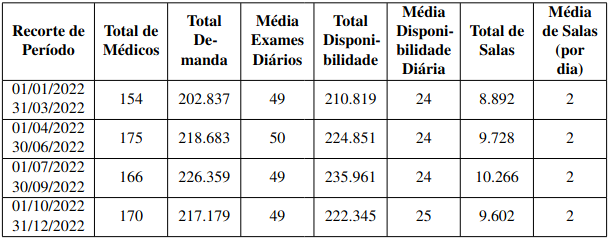
\includegraphics[width=1\linewidth]{img/quadro-instancia-dados.png}
        \caption{Informações por recorte trimestral}
        \label{fig:quad-recorte}
    \end{figure}
\end{frame}

\begin{frame}{Indicadores da Solução}
    \begin{figure}
        \centering
        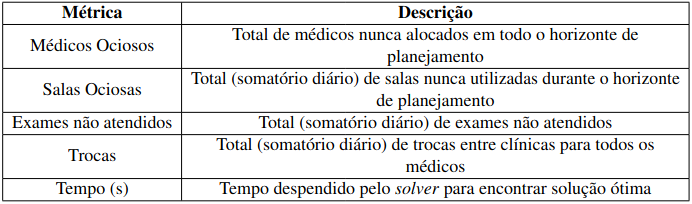
\includegraphics[width=1\linewidth]{img/criterios-avaliacao.png}
        \caption{Indicadores utilizados para avaliar as soluções entre si}
        \label{fig:criterios-avaliacao}
    \end{figure}
\end{frame}

\begin{frame}{Teste Computacional}
    \begin{block}{}
        \begin{itemize}
            \item \textit{Python} 3.12
            \item \textit{Gurobi} 12
            \item Ambiente Debian em plataforma Intel E5-2670V3
            \item 8 núcleos / 16 threads
            \item 8GB RAM
        \end{itemize}
    \end{block}
\end{frame}

\begin{frame}{Resultados Gerais}
    \begin{figure}
        \centering
        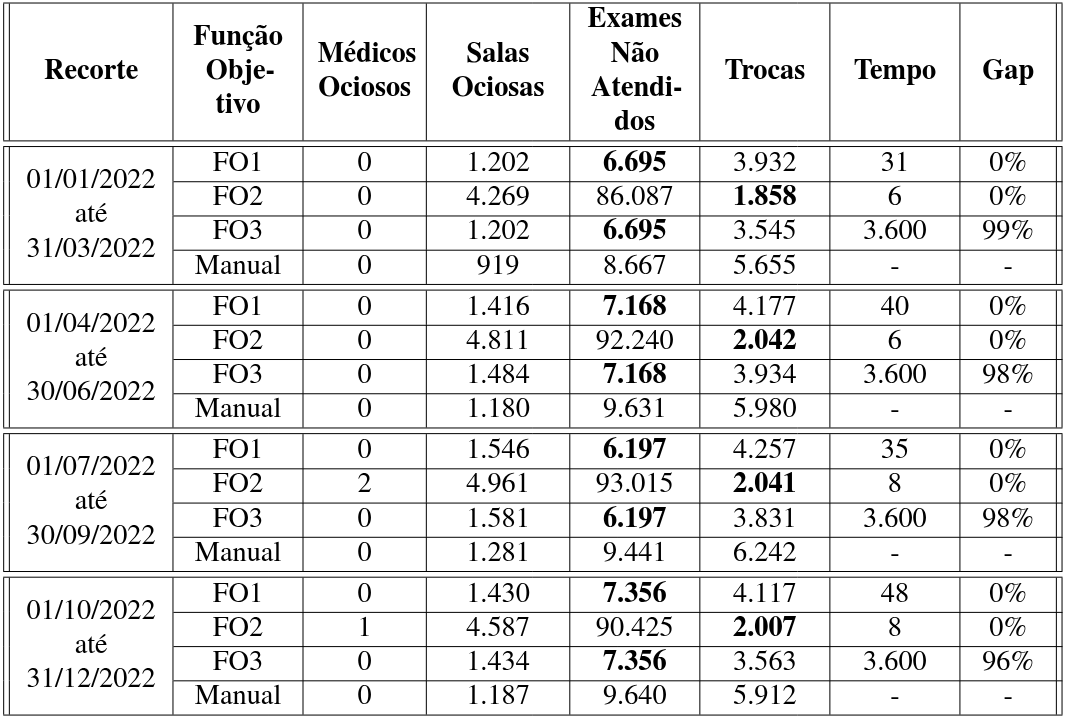
\includegraphics[width=0.85\linewidth]{img/resultados-gerais.png}
        \caption{Tabela de resultados do teste}
        \label{fig:resultados-gerais}
    \end{figure}
\end{frame}

\begin{frame}{Análise de Caso - FO1}
    
    \begin{footnotesize}

    \begin{block}{Pontos principais}
        Baixa uniformidade, altas trocas, foco em ocupação
    \end{block}
        
    \begin{minipage}[t]{0.475\textwidth}
        \begin{figure}
            \centering
            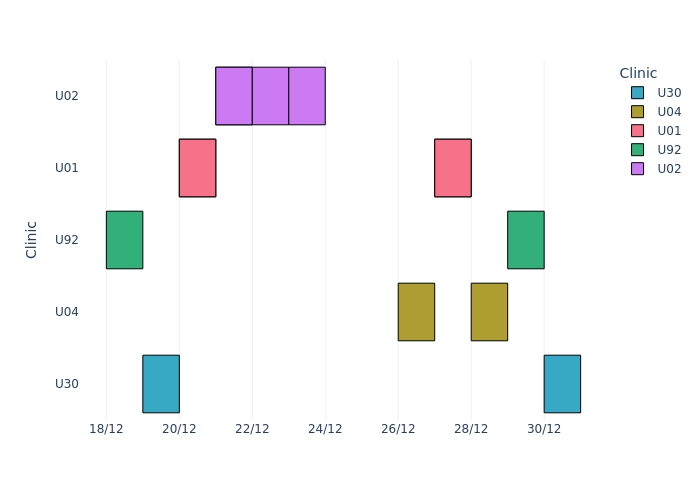
\includegraphics[height=3cm]{img/gantt_fo1.png}
            \caption{Agenda do médico}
            \label{fig:gantt-fo1}
        \end{figure}
    \end{minipage}
    \hfill
    \begin{minipage}[t]{0.475\textwidth}
        \begin{figure}
            \centering
            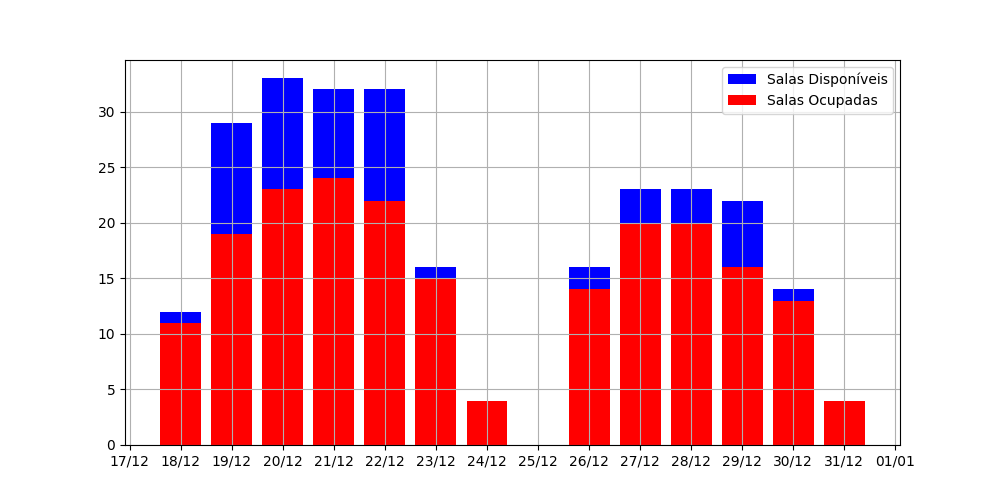
\includegraphics[height=3cm]{img/ocupacao-fo1.png}
            \caption{Ocupação de Salas}
            \label{fig:ocupacao-fo1}
        \end{figure}
    \end{minipage}

    \end{footnotesize}

\end{frame}

\begin{frame}{Análise de Caso - FO2}
    
    \begin{footnotesize}

    \begin{block}{Pontos principais}
        Agenda esparsa, ocupação mínima
    \end{block}
        
    \begin{minipage}[t]{0.475\textwidth}
        \begin{figure}
            \centering
            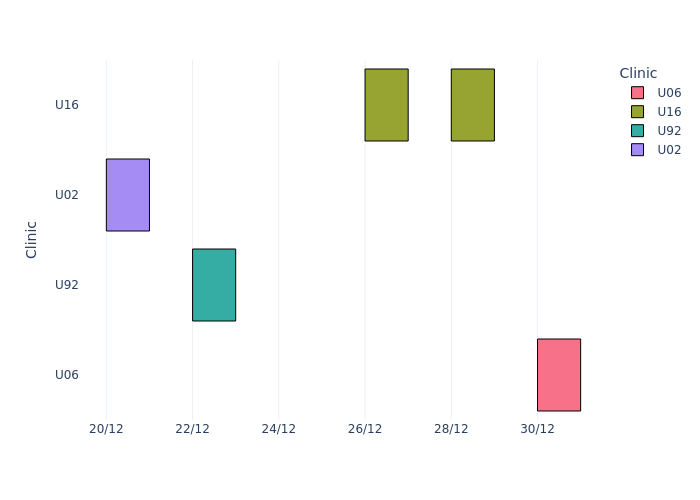
\includegraphics[height=3cm]{img/gantt_fo2.png}
            \caption{Agenda do médico}
            \label{fig:gantt-fo2}
        \end{figure}
    \end{minipage}
    \hfill
    \begin{minipage}[t]{0.475\textwidth}
        \begin{figure}
            \centering
            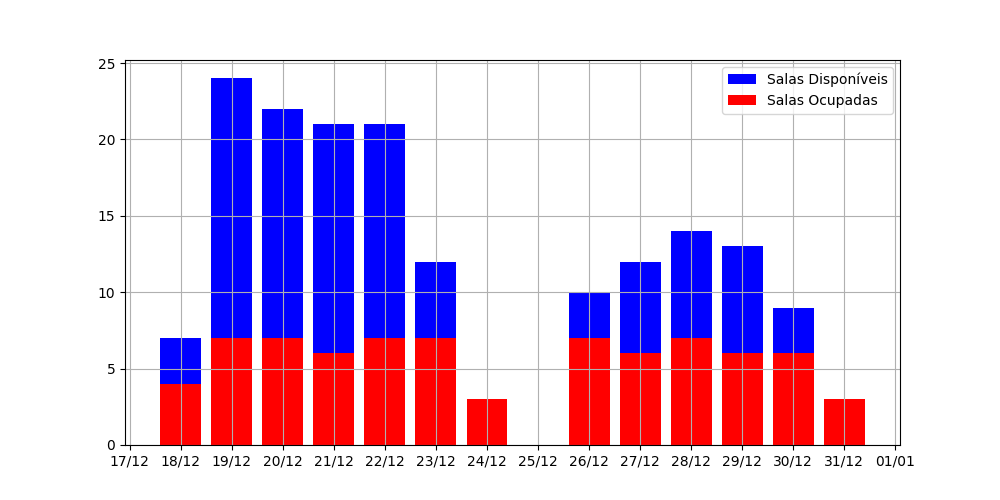
\includegraphics[height=3cm]{img/ocupacao-fo2.png}
            \caption{Ocupação de Salas}
            \label{fig:ocupacao-fo2}
        \end{figure}
    \end{minipage}

    \end{footnotesize}

\end{frame}

\begin{frame}{Análise de Caso - FO3}
    
    \begin{footnotesize}

    \begin{block}{Pontos principais}
        Agenda menos esparsa com boa ocupação
    \end{block}
        
    \begin{minipage}[t]{0.475\textwidth}
        \begin{figure}
            \centering
            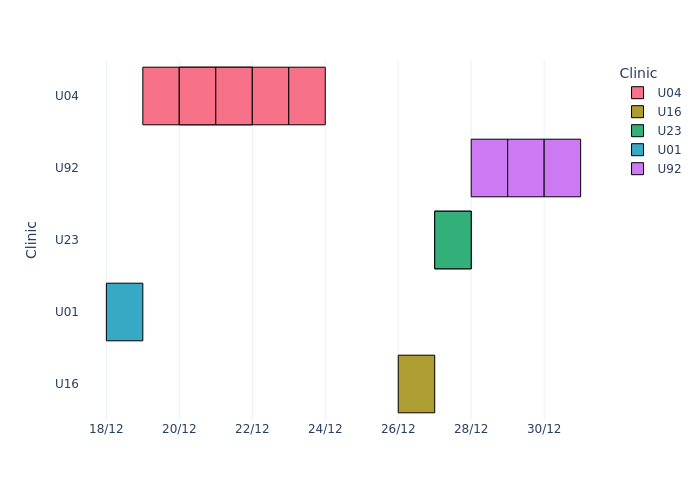
\includegraphics[height=3cm]{img/gantt_fo3.png}
            \caption{Agenda do médico}
            \label{fig:gantt-fo3}
        \end{figure}
    \end{minipage}
    \hfill
    \begin{minipage}[t]{0.475\textwidth}
        \begin{figure}
            \centering
            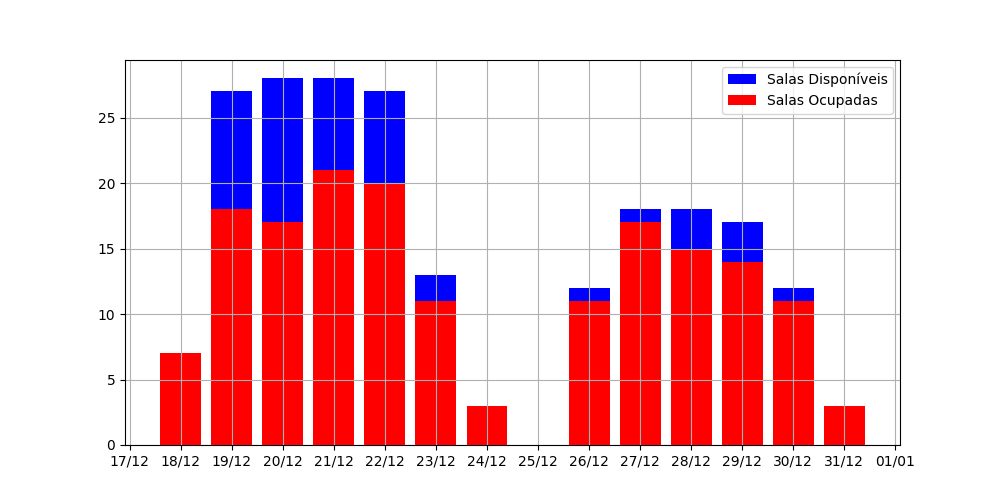
\includegraphics[height=3cm]{img/ocupacao-fo3.png}
            \caption{Ocupação de Salas}
            \label{fig:ocupacao-fo3}
        \end{figure}
    \end{minipage}

    \end{footnotesize}

\end{frame}